\section{Monte Carlo Simulation}
It has been already mentioned, that MC approaches can be used to research many body systems which are not solvable analytically.
Numerical methods simplify this task, but they introduce other challenges - in most cases (especially for large scaling sizes), it is not possible to acces every single state.
However, for the explanation of the used algorithm, this can be neglected for now.

\subsection{Detailed Balance and the Metropolis Algorithm}
Consider the particle flow out of state $\ket{i}$
\begin{align}
	j^\text{out}_{i} \mathrel{\mathop:}= \sum_j P_i(t) W_{ij},
\end{align}
with jump probability $W_{ij}$ from state $\ket{i}$ to $\ket{j}$.
Analogue, the particle flow into state $\ket{i}$ can be written as
\begin{align}
	j^\text{in}_{i} \mathrel{\mathop:}= \sum_j P_j(t) W_{ji}.
\end{align}
This yields to the master equation
\begin{align}
	\frac{\mathrm{d}P_i(t)}{\mathrm{d}t} = 
		\sum_{j}\left(P_j(t)W_{ji} - P_i(t)W_{ij}\right),
\end{align}
which is fulfilled in the equilibrium (left hand side vanishs) by the stricter condition of detailed balance\footnote{This is a strong, but not necessary condition to prevent the resulting Markov chain to be trapped in a limit cycle~\cite{newman1999monte}.}
\begin{align}
	P_iW_{ij} = P_jW_{ji}.
\end{align}
In other words - the system moves towards equilibrium if detailed balance is enforced\footnote{But not in the classical, newtonian way of motion, every snapshot of the system towards equilibrium is the result of random initialised trial steps.}.
The key of success is to choose $W_{ij}$ such that detailed balance is fulfilled.
This is accomplished with the Metropolis Criterion
\begin{align}
	W_{ij} = \left\{
		\begin{array}{c l}
			\exp(-\beta\Delta E)&\text{, if}\Delta E = E_j - E_i > 0\\
			1										&\text{, if }\Delta E \leq 0 
		\end{array}\right..
\end{align}
The according proof is short accepting $\Delta E > 0$ without qualification
\begin{align} 
	\frac{W_{ij}}{W_{ji}} = \frac{\exp\left(-\beta\Delta E\right)}{1} = \frac{\exp(-\beta E_j)}{Z}\cdot\frac{Z}{\exp(-\beta E_i)} = \frac{P_j}{P_i}.
\end{align}

\subsubsection*{Explanatory Note}
This criterion does always accept the trial state, if the energy is lowered and exponentially suppresses those, which raise the energy.
For the sake of illustration, all simulation steps will be described in detail.
\begin{enumerate}
	\item{Initialise the coordinates of all particles in a crystal}
	\item{Perform Monte Carlo moves with an acceptance of roughly \SI{60}{\percent}, i.e.
		\begin{itemize}
			\item{Select a particle and move it with vector $\delta \bm r$}
			\item{Compute the energy difference $\Delta E = E_j - E_i$}
			\item{Generate a uniformly distributed random number $x$ in $[0, 1]$ and accept the trial move, if eighter $\Delta E>0$ or $x < \exp(-\beta\Delta E)$, discard otherwise}
			\item{Repeat the previous steps $N$ times, assuming $N$ is the number of particles}
		\end{itemize}
	\item{In cases where the success ratio of movements is lower than \SI{60}{\percent}, adjust the length of $\delta r$ and try again.}
}
\end{enumerate}

\subsection{Implementation Characteristics}
One has to choose the algorithms parameters with caution - to access a good amount of states, the steps must show ergodicity.
For this purpose, the Monte Carlo step vector $\delta \bm r$ is a uniformly distributed vector on a sphere with norm $\left|\delta\bm r\right| = \epsilon$ per construction\footnote{Uniformly distributed $u=\cos(\theta)$ and $v=\phi$, the resulting vector via spherical coordinates.}.
% The mean movement of each particle now vanishes in equilibrium states.
In order to avoid unwanted divergencies, a sc lattice with equal distance between each particle pair is implemented as initial state.
The reason for choosing an acceptance ratio of \SI{60}{\percent} lies within the correlation of quantity measurements.
Taken the energy, for a $4\times10^4$ sample after $10^5$ MC-Steps, the correlation length differs according to the acceptance ratio (see Fig.~\ref{fig:MCCorrSeries}).
\begin{figure}[ht]
	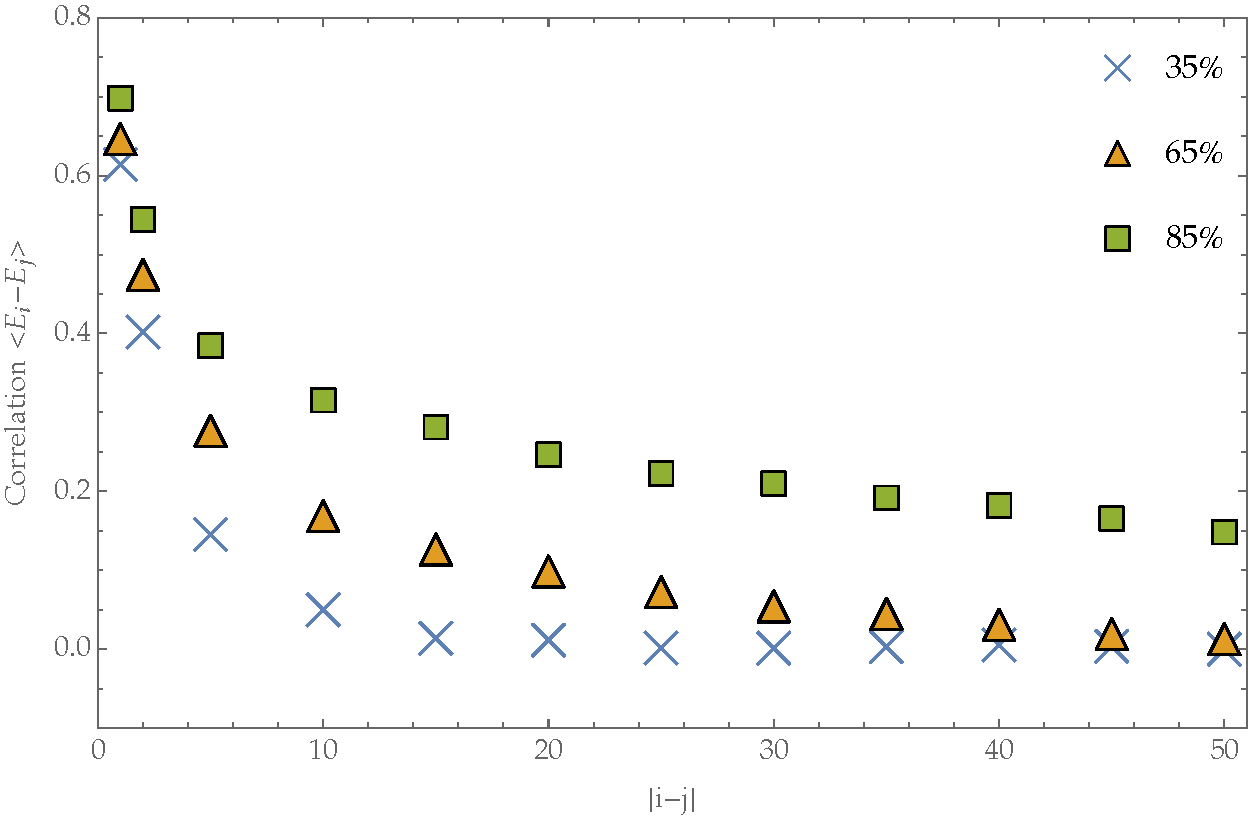
\includegraphics[width=\textwidth]{Figures/MCEnergyCorrelations.pdf}
	\caption[MC: Energy Correlation Series]{Energy correlation for a $4\times10^4$ sample. According to the acceptance ratio, the correlation length differs - also the shape of the correlation.}
	\label{fig:MCCorrSeries}
\end{figure}\\
To use nearly uncorrelated data for a meaningful quantity of interest, a smooth exponentially-decreasing correlation series and a sample distance of approximately $150$ MC-Steps has to be favored.
In principle - one has to analyse the correlation for each measurement in particular and decide which parameters are best, but due to time frame limitations, the fixed setting is listed in Tab.~\ref{tbl:MCSettings}.
\begin{table}[ht]
	\centering
	\begin{tabular}{l | l}
		System specifics &Setting \\
		\hline
		Number of particles &chosen according to density and system size\\
		Acceptance ratio&roughly set $\approx$ \SI{60}{\percent}\\
		Equilibration&after $2\times10^6$ MC-Steps\\
		Quantity series&$6\times10^3$ samples with $150$ MC-Steps distance\\
	\end{tabular}
	\caption[MC: Settings]{Listing with settings for the measurement via Monte-Carlo.}
	\label{tbl:MCSettings}
\end{table}

\subsection{Snapshots at Different Phase Points}
The next section is about different points at the phase diagramme.
